\documentclass[10pt,a4paper]{report}
\usepackage[margin=1.25in]{geometry}
\usepackage[pdftex]{graphicx}
\usepackage{subfigure}            % Multiple figures per float
\usepackage{placeins}             % Fix float loactions with \FloatBarrier
\usepackage{color}                % Color definitions for boxes
\usepackage{multirow}             % Multiple rows per cell in a table
\usepackage{verbatim}             % Long verbatim sections
\usepackage{titlesec}             % Easy modification the chapter format
\usepackage{fancyhdr}             % Easy modification of header and footer
\usepackage{hyperref}				% Custom hyperlinks
\usepackage{tikz}					% Figures and trees
\usetikzlibrary{arrows,shapes,positioning,shadows,trees}

\renewcommand{\arraystretch}{1.2} % Extra space in tables
\parindent0mm                     % New paragraphs start without indentation
\setlength{\parskip}{1em}         % And with a blank line in between

\tikzset{
  basic/.style  = {draw, text width=2.5cm, drop shadow, font=\sffamily, rectangle},
  root/.style   = {basic, rounded corners=2pt, thin, align=center,
                   fill=green!30},
  level 2/.style = {basic, rounded corners=6pt, thin,align=center, fill=green!60,
                   text width=10em},
  level 3/.style = {basic, thin, align=left, fill=blue!30, text width=8em},
  level 4/.style = {basic, thin, align=left, fill=blue!60, text width=8em},
  level 5/.style = {basic, thin, align=left, fill=gray!60, text width=10em}
}

% Redefine chapters to remove the "Chapter" word
\titleformat{\chapter}
  {\normalfont\LARGE\bfseries}{\thechapter}{1em}{}
\titlespacing*{\chapter}{0pt}{3.5ex plus 1ex minus .2ex}{2.3ex plus .2ex}

% Setup hyperlink format in document
\hypersetup{
    colorlinks=true, %set true if you want colored links
    linkcolor=blue,  %choose some color if you want links to stand out
    citecolor=blue,  %choose some color if you want lcitation to stand out
    filecolor=black, % etc...
    urlcolor=blue
}

% Define header and footer
\pagestyle{fancy}
\fancyhf{}
\lhead{C. Rosales, A. G\'{o}mez}
\rhead{REMORA User Guide}
\lfoot{REMORA User Guide}
\rfoot{\thepage}

% Define header and footer for first page in chapter
\fancypagestyle{plain}{
\fancyhf{}
\lhead{C. Rosales, A. G\'{o}mez, C. -Y. Lu, K. Milfeld}
\rhead{REMORA User Guide}
\lfoot{REMORA User Guide}
\rfoot{\thepage}
}

% Gray boxes for optional material
\definecolor{LightGrey}{gray}{.85}
\setlength{\fboxrule}{1pt}
\setlength{\fboxsep}{6pt}
\newcommand{\IntroBox}[1]{
  %\fcolorbox[rgb]{0,0,0}{0.95,0.95,0.95}{
    \fcolorbox{black}{LightGrey}{
    \begin{minipage}{0.94\linewidth}
      %\textbf{Introduction}
      #1
    \end{minipage}
  }
}


%Chun-Yaung Lu and Kent Milfeld. ``REMORA Resource Monitor: Usability, Performance and User Interface Improvements''.


\begin{document}

\begin{titlepage}
\thispagestyle{empty}	%don't include number on cover
%\begin{flushleft}
%\begin{figure}
%\includegraphics[width=0.2\textwidth]{gplv3-127x51.png}
%\end{figure}
%\end{flushleft}
\verb+ +
\vspace{1em}
\begin{flushright}
\huge\bf REMORA v2\\
\rule{\textwidth}{4pt}
\large{\bf REsource MOnitoring for Remote Applications\\
Document Revision 1.0\\
\today}
\end{flushright}

\begin{figure}[ht!]
	\centering
	\includegraphics[width=0.5\columnwidth]{logos/Remora-logo-600px.png}
\end{figure}

%Back of cover page (copyright)
\newpage
\thispagestyle{empty}
\begin{flushleft}
Antonio G\'omez-Iglesias, Carlos Rosales Fern\'andez (Version 1)\\
\verb+agomez@tacc.utexas.edu+, \verb+carlos@tacc.utexas.edu+\\
\vspace{0.5em}
Chun-Yaung, Kent Milfeld (Version 2)\\
\verb+cylu@tacc.utexas.edu+, \verb+milfeld@tacc.utexas.edu+\\

\vspace{0.5em}
High Performance Computing \\
Texas Advanced Computing Center\\
The University of Texas at Austin\\
\vspace{1cm}
Copyright 2023 The University of Texas at Austin.
\end{flushleft}
\newpage
\end{titlepage}

\begin{abstract}

REMORA is a modular tool to monitor a job runtime resource utilization in HPC environments. 
As of version 2.0 the suite contains code designed to test:

\begin{itemize}
\item Memory utilization in CPUs, Xeon Phi co-processors, and NVIDIA GPUs
\item CPU utilization
\item IO utilization for the Lustre and DVS file systems
\item NUMA properties
\item Network topology
\item MPI communication statistics
\item Socket Power consumption
\item CPU temperature
\end{itemize}

Throughout the text we have used text boxes to highlight important information. These boxes look like this:

\IntroBox{These gray boxes contain highlighted material for each section and chapter.}

Remora was designed to provide a runtime resource monitoring tool that is both simple to use
and presents easy to understand high level information of resource usage, as well as detailed statistics for in-depth analysis. 
We welcome all feedback, particulary suggestions that  includes improvement in the usability, reliability, 
and accuracy. 

Version 2.0 is a feature release that has been optimized to reduced collection overhead, programmed for attachment to
running jobs, power collection for all intel platforms (with rapl), provide easier control over 
resource module selection, and support unit testing.

REMORA is an open-source project.  Please help support continued development/improvement by citing Remora:

C. Rosales, A. G\'{o}mez-Iglesias, A. Predoehl. ``REMORA: a Resource Monitoring Tool for Everyone''. HUST2015 November 15-20, 2015, Austin, TX, USA. DOI: 10.1145/2834996.2834999 \cite{remora}

Chun-Yaung Lu and Kent Milfeld. ``REMORA Resource Monitor: Usability, Performance and User Interface Improvements''.
 HUST2023 November 15-20, 2023,, USA. DOI: 10.1145/2834996.2834999 \cite{remora}
\end{abstract}

\tableofcontents

\chapter{Installation}
REMORA is simple to install. 
In order to use all of its features you will need GNU Make and a C compiler. 
Support for MPI statistics requires an MPI installation with an MPI compiler wrappers and runtime.

Download the latest tar version from the following URL in your  browser:
\footnote{\href{https://github.com/tacc/remora/tarball/master}
{https://github.com/tacc/remora/tarball/master}} 
and extract the contents in your system:

\begin{verbatim}
    tar xvf *remora*.tar
\end{verbatim}

Alternatively clone the git repository with the latest development version (not recommended):

\begin{verbatim}
    git clone https://github.com/TACC/remora
\end{verbatim}

This will create a top level directory called \verb+remora+, 
with subdirectories \verb+/docs+, \verb+/extra+ \verb+/src+. 
Change directory to remora and edit \verb+install.sh+ to reflect your choice of installation directory, build type, and modules configuration. The variables to modify are:

\begin{table}[h]
\centering
\label{tab:env}
\begin{tabular}{|l|l|l|}
\hline
\bf{Variable}	& \bf{Description}                          & \bf{Default}\\\hline
REMORA\_DIR     & Absolute path to installation directory   & . \\\hline
\end{tabular}
\end{table}

The resource data collectors, modules, are configured in the \verb+src\config\modules+ file. 
Simply remove any modules that you don't want to be available in your system. 
Also, you can create your own modules and add them into this file.
(See Section \ref{expand-remora} for more information about how to expand REMORA's functionality).

By default Remora is installed in the present working directory (\verb+remora+).
Change compiler variables in the install script, install.sh; also the install directory
can be set by directly assigning a path to \verb|REMORA_DIR|.
(\verb|REMORA_INSTALL_PREFIX|, PWD is the default) in install.sh.
Then, execute install.sh to build and install remora.

\begin{verbatim}
    ./install.sh |& tee install.log
\end{verbatim}

An installation path can also be specified on the command line:
\begin{verbatim}
    REMORA_INSTALL_PREFIX=<install_directory> ./install.sh |& install.log
\end{verbatim}

\section{More on MPI Support}
If your systems supports multiple MPI stacks you should build a version 
for each of stack, since the collection of MPI statistics is performed differently for each stack.
The installation script will detect and set the mpiexec and 
mpicc / mpif90 compilers of the present environment.
Simply use a different installation prefix for each of the 
stacks so the installations do not overwrite each other. 
When no MPI compiler is present during the installation, remora will be installed with 
full functionality except for the missing MPI statistics support.
%%KFM  check how to do this easier.

After installing remora, make sure the remora \verb+bin+ directory is prepended to your \verb+PATH+ 
and the remora \verb+lib+ directory is in your \verb|LD_LIBRARY_PATH|. 
(Remora determines the \verb+bin+ path from your PATH variable, sets \verb|REMORA_BIN| to its 
value and uses the variable in remote processes to specify the location of remora execution scripts.) 

For SH/BASH/ZSH users, add the follow to an appropriate startup file to ensure REMORA 
is available every time you login. 
\begin{verbatim}
	export PATH=$REMORA_DIR/bin:$PATH
	export LD_LIBRARY_PATH=$REMORA_DIR/bin/lib:$LD_LIBRARY_PATH
\end{verbatim}

If the mkmod utility is installed on your system, after installation, cd to the install
directory (where bin exists), and execute the follow to create a my\_remora user-space module:
\begin{verbatim}
	module load mkmod 
	export NAME=remora VER=2.0 TOPDIR=`pwd` 
        mkmod
\end{verbatim}
After this, the command module load my\_remora will create an execution environment for you
(with the correct PATH, LD\_LIBRARY\_PATH, and module help information).

\FloatBarrier
\chapter{Using REMORA}

\section{Collecting Data with remora Wrapper}

If you are on a system that manages application environments with modules, load remora:
\begin{verbatim}
      module load remora
\end{verbatim}
Otherwise, it is assumed that the remora command and library are in your PATH and LD\_LIBRARY\_PATH
variables, respectively.

For a serial job:

\begin{verbatim}
        export REMORA_PERIOD=2     #change default period from 10 sec. to 2
	remora app [app_args]
\end{verbatim} 

For a parallel job (assuming \verb+mpirun+ is your parallel launcher, change for mpiexec.hydra, ibrun or other as needed):

\begin{verbatim}
	remora mpirun [mpirun_options] mpi_app [mpi_app_args]
\end{verbatim} 

The code will run as normal, and contain remora summary printed to stdout at the end. 
Also, a directory named \verb+remora_<jobid>+, where \verb+jobid+ is the job number, 
will contain remora data files (*.txt) and an html index file (remora\_summary.html)
linking to the Google Charts (*.html), that you can open on your laptop
to view the resource usage. Currently SGE and SLURM are supported.

\begin{table}
\begin{center}
\begin{tabular}{|l|l|}
\hline
\bf{Directory} & \bf{Contents}\\\hline
CPU	      & CPU utilization\\\hline
INFO      & Runtime environment and hostlist\\\hline
IO        & File system utilization\\\hline 
MEMORY    & Memory utilization\\\hline
MONITOR   & Continuous monitoring data (MONITOR mode only)\\\hline
NETWORK   & IB utilization data\\\hline
NUMA      & Non-Uniform Memory Access data\\\hline
POWER     & Power consumption\\\hline
TEMPERATURE & CPU temperature\\
\hline
\end{tabular}
\label{tab:outdir}
\caption{Contents of output directory}
\end{center}
\end{table}

The Remora output directory will contain a set of subdirectories with information 
about different resources used by your code -- See table \ref{tab:outdir} -- 
as well as a summary output in your terminal screen (interactive use) or stdout file (batch use). 
An example of the summary output is shown in Figure \ref{fig:summary}.

The summary shown in Figure \ref{fig:summary} shows that the maximum 
virtual and physical memory 
used per node in this particular execution was 6.08 GB and the executable ran 
for just over 55 seconds, with 14\% of the total execution time spent in MPI 
routines (inclusive of communication and MPI IO). 
From the output we can also see that the job was run out of the \verb+scratch+ 
file system, and that very small amounts of IO occurred throughout the execution. 
As indicated by the \verb+Sampling Period+ entry data was collected using a 
\verb|REMORA_PERIOD| of 2 seconds, and the complete collected data set can be 
found in the \verb+remora_5599286+ directory. The maximum IO was 42 MB/s with
only 68 IOPS maximum.
This summary information is saved in \verb+remora_5599286/INFO+ directory.

\begin{figure}
\begin{verbatim}
=============================== REMORA SUMMARY ===============================
 Max Virtual  Memory Per Node :     6.08 GB
 Max Physical Memory Per Node :     1.23 GB
 Available Memory at time 0.0 :   177.56 GB
 MPI Communication Time       :    13.95 %
 Total Elapsed Time           :  0d 0h  0m 55s 276ms
------------------------------------------------------------------------------
 Max IO Load / home1          :      68 IOPS      42 RD(MB/S)       0 WR(MB/S)
 Max IO Load / scratch        :      70 IOPS       1 RD(MB/S)       0 WR(MB/S)
 Max IO Load / work           :       1 IOPS       0 RD(MB/S)       0 WR(MB/S)
==============================================================================
 Sampling Period              : 2 seconds
 Report Directory             : R=/scratch/00770/milfeld/amber/remora_5599286
 Google Plots HTML Index Page : $R/remora_summary.html
==============================================================================
\end{verbatim}
\caption{Summary output for typical job execution using REMORA}
\label{fig:summary}
\end{figure}

\FloatBarrier
\section{Execution Customization}\label{customize}

REMORA is configurable in terms of the amount and type of data collected, but sensible defaults are provided to simplify its use. By default the resource data are collected every ten seconds.

REMORA provides two different running modes and it also allows the users to specify how frequently the data is collected. A verbose mode is provided mostly for troubleshooting and should not be used by default. The behavior of the application is controlled via four environment variables:

\IntroBox{
\begin{itemize}
	\item \texttt{REMORA\_MODE}: this variable accepts three possible values (BASIC, FULL, and MONITOR). The FULL mode runs all the tests that the tool allows. The BASIC mode only reports memory and cpu usage. MONITOR mode is equivalent to FULL, with the added advantage that data is post-processed inline and a summary file is generated in real time for application monitoring. BASIC is the recommended mode when the users know that the application of interest does not create problems in the distributed file system. The default is FULL.
	
	\item \texttt{REMORA\_PERIOD}: Time in seconds between consecutive data records. This is the time from the end of a collection event until the start of the next collection event. Depending on the platform where the tool is running, the overhead introduced by the application can make the duration of the collection event to vary, in which case there will be less data points in the collected results than expected. However, in the systems that we have tested the overhead of the application is small enough that the total number of collection points (CP) is almost equal to $CP = ET/RP$ where ET is the execution time (in seconds) and RP is the period (in seconds).
	
	\item \texttt{REMORA\_MONITOR\_PERIOD}: Similar to \texttt{REMORA\_PERIOD}. It corresponds to the number of seconds between updates to the monitor file which contains the real time summary of resource utilization. This is provided in case regular monitoring data is required at a different rate than the full data collection. It must always be larger than \texttt{REMORA\_PERIOD}.
	
	\item \texttt{REMORA\_TMPDIR}: Full path for intermediate file storage. It is recommended that this is a local disk. Default value is the location of the REMORA output directory (which must be on a shared file system). When specified by the user REMORA will collect data in this location, and only copy the files to the output directory once data collection is complete. Using a local file system for the temporary files reduces overhead. 

    \item \texttt{REMORA\_PLOT\_RESULTS}: When this variable is unset, by default, REMORA automatically generates a set of HTML files with plots for the collected data. However, for very large use cases, this automatic generation can take a long time. Users can skip the generation of these files by setting this variable to 0. A value of 1 designates automatic generation.

	\item \texttt{REMORA\_VERBOSE}: Enable (1) or disable (0) verbose mode. Default is disabled.
	
	\item \texttt{REMORA\_WARNING}: Verbosity level for REMORA issued warnings. Acceptable values are 0, 1, 2 in increasing level of verbosity. Critical errors will always be reported independently of the chosen value.
\end{itemize}
}

In addition to these variables a list of file systems that should be ignored during data collection can be provided to REMORA in the file \verb+config/fs_blacklist+. This is a simple text file with a names of mounts that should be ignored during runtime.

\section{Collecting Data with snapshot, after attachment}

The \verb+snapshot+ command is used to gather remora data from a running job.
After accessing (attaching to) a compute node of a running job (with ssh), load the remora module
and execute \verb+snapshot+ in its simplest form, with the number of data points (required) 
to be collected. To collect 100 snapshots (data values) for the default period, execute:
The number of snapshots is required.

\begin{verbatim}
	snapshot 100
\end{verbatim}

The command has options that allow a user to set the period (an integer) on the
command line (or set the REMORA\_PERIOD env. var.).  Also, The arguments
can be a list of the collection modules to use. No order is required, except
for the number of snapshots, which must be first.

\begin{verbatim}
	snapshot num_snapshots [period] [space-separated list of modules]
  e.g.
	snapshot 100  10 memory mpi   #100 snapshots 1_snapshot/10sec 
                                      #collect only memory and mpi info
\end{verbatim}

By default, data is collected for all nodes in a job.  Use the argument \verb+node+
to just collect data for the node you are presently accessing. Also, by default
plots are not created for a snapshot execution.  

The plots are not automatically generated in \verb+snapshot+ because plots are
created on each node, and will compete with the execution of your job. 

If this is of no concern, add the \verb+plot+ to the  snapshot command to create
plots immediately after data collection.

\section{Plotting snapshot data}

After collecting data from \verb+snapshot+, execute \verb+snapshot+ with 
\verb+plot+ as the first argument on a login node in the directory where 
the snapshots were taken:

\begin{verbatim}
	snapshot plot         #execute on login node, remora_<job_id> in PWD
or
	snapshot plot remora_<job>      #supply remora_<job_id> path
\end{verbatim}

When plotting the snapshot data, the data in the latest remora directory 
(remora\_<job\_id>) in the present working (top level) directory is found and used for the plots.
A different remora\_<job\_id> may be suppliede,
or a full path to a remora\_<job\_id> directory can be added as an argument 
if the present working directory is not a top level directory.

\section{Post-Processing}
All the data is collected in a set of files with the metrics organized in columns. 
Since remora data consists of ASCII files, with space separated column data, 
with each row pre-pending with a time stamp,
it is easy to extract remora data with your own postprocessing tools. 
However, for simplicity, REMORA already provides a plotting script called 
\verb+remora_post+ that takes all the metrics generated during collection and generates plots. 
These plots show the most relevant information previously collected and 
represent a visual alternative while analyzing the results. 
The script can be called from the batch script or from the login nodes after the job has finished. 
In this second scenario, the script requires an argument with the job ID to be analyzed.

The post-processing script can be invoked simply as:

\begin{verbatim}
	remora_post -j <jobID>
\end{verbatim}

\section{Post-Crash Summary}
In a typical situation, when an application crashes, the remora collection is interrupted and
no final summary is produced (or an incomplete summary is shown).
We now provide an independent script \texttt{remora\_post\_crash} that attempts to produce 
a final summary of the collected data. This script can be executed as:

\begin{verbatim}
	remora_post_crash <JobID>
\end{verbatim}

\section{Automated Memory Protection}
Following user requests we have developed a simplified version of remora that does not produce any data collection records but simply monitors application memory usage and kills the user application if available memory on each node reaches a minimum threshold.

For a serial job:

\begin{verbatim}
	remora_mem_safe ./myexe [myexe_arguments]
\end{verbatim} 

For a parallel job (assuming \verb+mpirun+ is your parallel launcher, change for mpiexec.hydra, ibrun or other as needed):

\begin{verbatim}
	remora_mem_safe mpirun [mpirun_options] ./myexe [myexe_arguments]
\end{verbatim} 

The minimum memory available is configured by default to be 0.5GB, and the sampling period is 0.01 seconds. 
The sampling period is not configurable, but the memory threshold can be modified.

\IntroBox{
\begin{itemize}
	\item \texttt{REMORA\_FREEMEM}: this variable sets the minimum available memory (in KB) for \texttt{remora\_mem\_free}. If available memory falls below this threshold all user processes under monitoring will be killed.
\end{itemize}
}
%%%%%%%%%%%%%%%%%%%%%%%%%%%%%%%% START HERE
\FloatBarrier
\chapter{Design and Implementation}
REMORA is designed with ease of use in mind. 
Use with minimal effort is fundamental throughout the model.
This is included in access, operation, employment of features, understanding collection tables and reports and visual presentations.
While there are models where the tool could run transparently, 
just by loading a module that would change the environment to collect all the information at runtime, 
we decided to opt for a model where the user loads the module, and then changes the submission script 
to invoke the remora tool by prepending its name to the actual command that has to be analyzed. 
This has the advantage of preventing unnecessary overhead when the module is loaded and runs 
that do not require instrumentation are submitted. 
It also simplifies the data collection for serial jobs and scripts, which do not use an MPI launcher 
that can be easily hijacked or modified. For example, if the original command is \textit{mpirun ./myparallelapp}, 
the new command will be \textit{remora mpirun ./myparallelapp}. 
A more complicated scenario is when the user wants to run a set of different commands or scripts in the same job. 
In that case, it is necessary to put all the commands to be executed in a shell script 
(i.e. a shell script called \textit{mycommands}). 
Then, executed the script with the remora wrapper: \textit{remora ./myjob}. 
Note, \verb+remora+ can be used in a batch script or interactively in the command prompt.

As a system-installed tool, the remora environment will be accessible by loading a Lua or Tcl resource module
(module load remora). Users can install their own version Remora.  
Users can create their own module (with mktau), or simply add environment setup commands to their startup shells
(the exact commands are listed at the end of the install).

In its current implementation the tool generates a flat ssh tree with a single connection from the master node in the execution to all other nodes. This connection initiates a background process that collects the statistics for each node with a frequency specified by the user. The remote background tasks execute a loop over all processes owned by the user, and aggregate the data before committing it to file.

For runs involving a Xeon Phi co-processor the background task is pinned to the last core (assumed to own hardware threads 0, 241, 242 and 243) since in most execution modes this will avoid interference with the application during runtime and minimize impact on the execution time. The source file \texttt{mic\_affinity.c} can be modified in order to change this setting.

In monitor mode, a subset of the metrics is appended to a file that the user tails in real time.

\section{Data Collection}
REMORA collects a set of metrics that is useful in many different scenarios when profiling and evaluating
resource usage of an application. The data collected by REMORA consist of:

\begin{itemize}
\item Detailed timing of the application.
\item CPU loads.
\item Memory utilization.
\item NUMA information.
\item I/O information (file system load and Lustre traffic).
\item Network information (topology and InfiniBand traffic).
\item MPI Statistics (time, most used MPI calls, message sizes)
\item Temperature (of each core)
\item Power (of each socket)
\end{itemize}

Dynamic information is collected every \texttt{REMORA\_PERIOD} seconds. The following describes the data collected in more detail. 

\paragraph{CPU}
The application reports the average CPU usage of the last second (independently of the value specified for \texttt{REMORA\_PERIOD}). This information is very important for applications that use OpenMP, where it is possible to easily analyze how the cores are being used. It also allows to check for a correct pinning of threads to the cores: not pinning processes could lead to threads floating between cores, which will be show up in this report. MPI applications can also benefit from this information.

\paragraph{Memory}
One of the most recurring questions for HPC users is "how can I know how much memory my job is using?". Trying to answer that question, REMORA collects the most relevant statistics regarding memory usage every \texttt{REMORA\_PERIOD} seconds (more information in Section \ref{customize}):

\begin{itemize}
\item Virtual Memory (and Max Virtual Memory): this is a very important value as the OOM (out of memory) killer will use it to kill the application if needed.
\item Resident Memory (and Max Resident Memory): physical memory used by the application.
\item Shared memory: applications have access to shared memory by means of /dev/shm. Any file that is put there counts towards the memory used by the application, so the application reports this usage.
\item Total free memory: this will take into account the memory not being used by the application, the libraries needed by the application, and the OS.
\end{itemize}

Data is collected from /proc/\textless pid\textgreater /status for all of these except shared memory, which can be obtained from /dev/shm. Memory usage for all user processes is aggregated and written to a single file per node involved in the execution. At the end of the run the maximum values for memory utilization (and minimum value of total free memory) are aggregated into a single file.

When Xeon Phi co-processors are used as part of a symmetric execution model, each Xeon Phi is treated as a separate node and the same memory information is collected from Phi and from host CPU. Individual files are maintained for each node and Phi and the per node aggregated summary is provided individually for nodes and Xeon Phi devices, since their available memory tends to be different.

\paragraph{NUMA}
As it is well known, NUMA (Non-Uniform Memory Access) can have a large impact on the overall performance of an application. Sometimes small changes in the code can lead to large improvements once it has been discovered that NUMA was imposing a penalty over the application. Our tool reports how memory is being used in each socket and it also collects the number of NUMA hits and misses. The information is extracted from the \texttt{numastat} tool: \texttt{numastat} is called only once on each collecting period; the output of \texttt{numastat} is then analyzed and several different fields are used for the statistics:

\begin{itemize}
	\item Number of hits: total number of memory access hits. 
	\item Number of misses: total number of memory access misses. 
	\item Number of hits in the current node: if the data that the application was looking for is in the same of node where the core requesting that data is located, it produces a hit in the current NUMA node.
	\item Number of hits in the other node: when the data required is in cache, but in the other NUMA node.
	\item Total memory free/used on each node.
\end{itemize}


\paragraph{Lustre} 

A new Lustre module was included in REMORA 1.4.0. This module looks at the content of the files located in \verb+/proc/fs/lustre/{mdc,osc}/*/+ . In particular, it looks for the content of the stats file. In order to generate a more user-friendly data, and it extracts the name of the filesystems and the different lustre mounts from the \texttt{df} command.

\paragraph{DVS}

A new Data Virtualization Service (DVS) module was added in REMORA 1.5.0. This module captures information in the \verb+/proc/fs/dvs/mounts/*/+ files to provide the number of requests per second for every DVS served file system that is not in the blacklist under \verb+/config/fs\_blacklist+.


\paragraph{LNET Stats}
Our tool collects information regarding the data transferred by Lustre on each node used by the job while running. Normally, these statistics do not provide much information to the users. However, they are very useful if there was a problem in the file system while the job was being analyzed, as the number of messages dropped will significantly increase. The following Lustre information is collected:

\begin{itemize}
\item Number of currently active Lustre messages. It also includes a highwater mark of this value.
\item Messages sent/received: total number of Lustre messages sent/received by the current node.
\item Messages dropped: number of Lustre messages that failed to be delivered to the destination.
\item Bytes sent/received: total number of bytes sent/received on Lustre messages.
\end{itemize}


\paragraph{InfiniBand Packets}
Number of packets transmitted using InfiniBand. This data can be used to get extra information regarding how the communication in parallel applications takes place. In particular, the time series can be used to correlate high network activity levels with sections of the code, and those ections can be revised for possible optimization.

\paragraph{MPI Statistics}
MPI statistics are collected using mpiP for Mvapich2 and the internal mechanisms for Intel MPI. The percentage of execution time spent in MPI calls is included in the summary report, and the raw data stored in the MPI/mpi\_data.txt file. A simple pie chart shows the percentage of time spent in MPI calls -- including communication and IO -- and a bar chart is provided showing the five MPI cals where the application spent most of its communication time.

%%%%%%%%%%%%%%%%%%%%%%%%%%%%%%%% UP Completed BELOW
\FloatBarrier
\section{Modular Design}
REMORA presents a modular design that makes it easy to modify and extend the functionality 
provided by the tool. For example, currently REMORA supports
the Lustre file system, but there are HPC systems that use other types of file systems.
Data collection for those file systems can be incorporated into REMORA in a straightforward
manner due to its modular design.

This design allows the automatic discovery of new functionality by means of a configuration
file that is read during REMORA startup. This configuration file contains
a list of module names to activate. Typically, each of these modules collects a 
different type of statistic. The tool will read each line and will load a
script file with the same name specified in the configuration file. The script file needs
to implement at least four functions: initialization, data collection, post-processing, and 
finalization.

Developers of new modules may define other functions,
but they will have to be called from one of the four required functions. The initialization,
post-processing and finalization functions are called only once during the execution of the
tool, while the data collection method will be called by REMORA on each time step.

If the default configuration file includes, for example, a line with the text \textit{cpu}.
This line indicates there will be a script with the file name \textit{cpu}. This script
is responsible for collecting the data regarding CPU utilization on each one of the
nodes used by the application. The script defines the following functions:

\begin{itemize}
	\item init\_module\_cpu
	\item collect\_data\_cpu
	\item process\_data\_cpu
	\item plot\_data\_cpu
	\item monitor\_data\_cpu
	\item finalize\_module\_cpu
\end{itemize}

Each of these functions takes three arguments: 

\begin{itemize}
\item Name of the node where the function is running      (\texttt{\$REMORA\_NODE})
\item Full path where the output will be stored           (\texttt{\$REMORA\_OUTDIR})
\item Full path to an optional temporary storage location (\texttt{\$REMORA\_TMPDIR})
\end{itemize}

\verb+$REMORA_NODE $REMORA_OUTDIR $REMORA_TMPDIR+

Because it isn't necessary to understand the program architeture and calling sequence 
to create a module which initializes, collects and plots data from a resource,
it is simple to extend REMORAS's functionality to
to  include additional resources.
All that is necessary is to create a
to create a new module file (named appropriately after the resource, here named \textit{newres\_module}) 
with the following functions:

\begin{itemize}
	\item     init\_module\_newres\_module
	\item    collect\_data\_newres\_module
	\item       plot\_data\_newres\_module
	\item    monitor\_data\_newres\_module
	\item finalize\_module\_newres\_module
\end{itemize}

Use any one of the other modules as a template.
In order to activate \emph{newres\_module}, include a line in the configuration file
with the text \textit{newres\_module}. Functions may be left empty (e.g. monitor\_data\_newres\_module). 
Typically, the majority of a module's functionality will be implemented in the data collection module.

This design also makes it straightforward to deactivate existing modules.
Simply by removing a module name in the configuration file, the module becomes disabled during a run.

\FloatBarrier
\section{Code Structure}

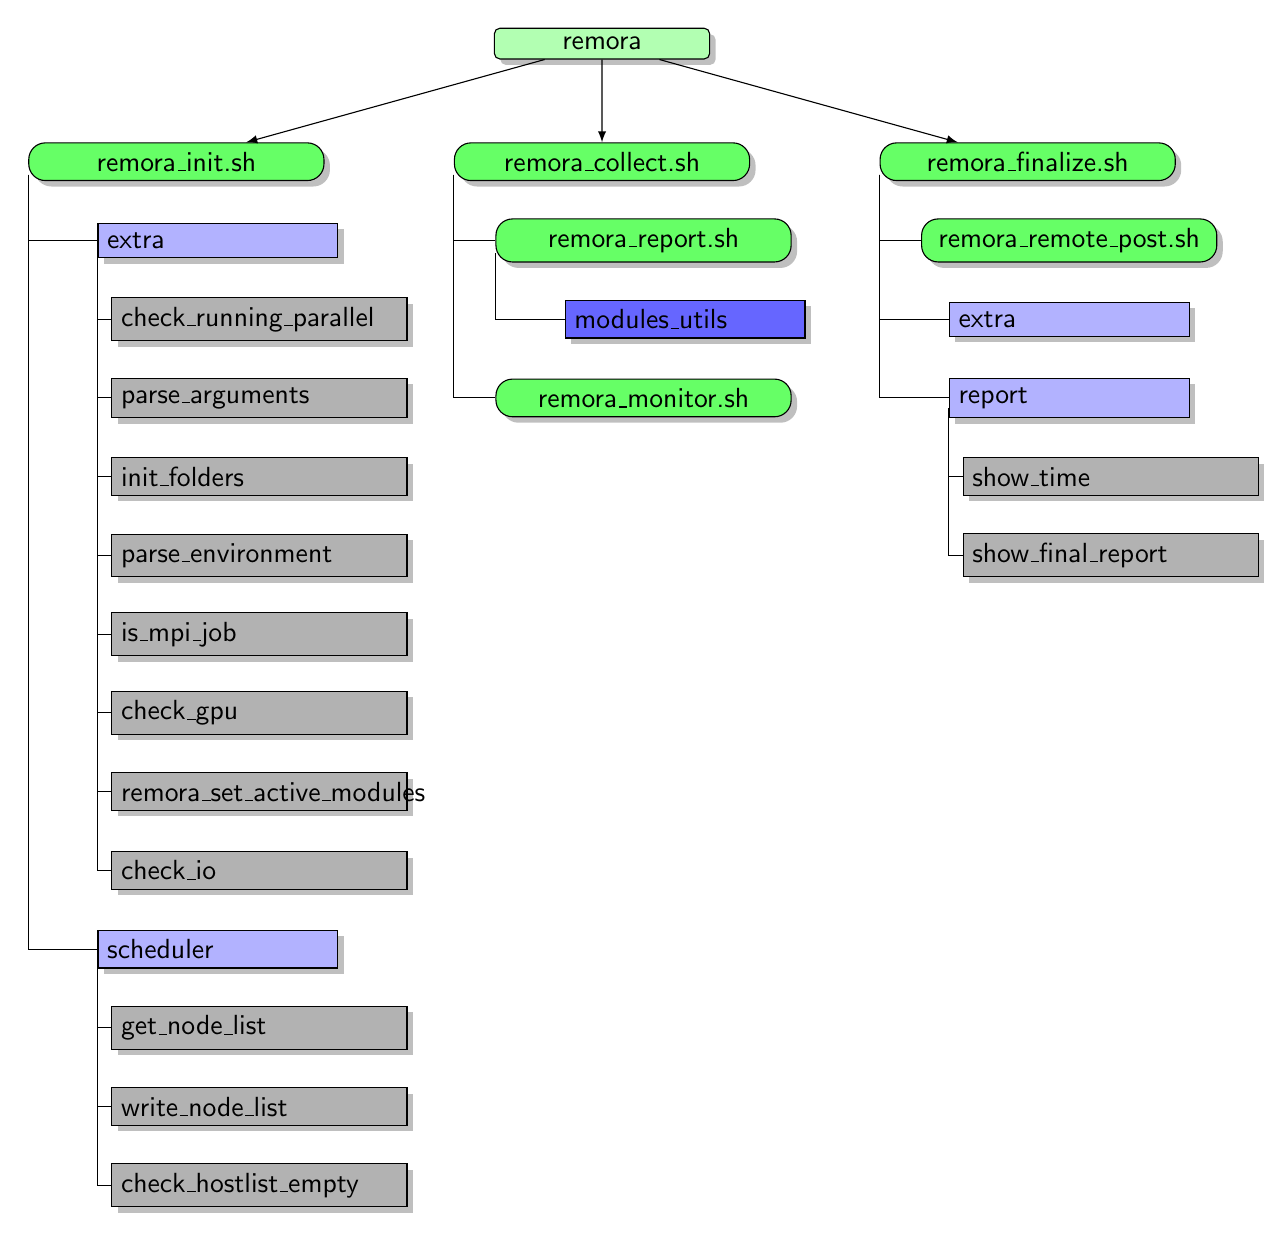
\begin{tikzpicture}[level 1/.style={sibling distance=40mm},edge from parent/.style={->,draw},>=latex]

% scripts are level 2, aux is level 3, modules is level 4, bash funcs are level 5

\node[root] { remora }
  child {node[level 2, xshift=-40pt] (c1) {remora\_init.sh} }
  child {node[level 2]               (c2) {remora\_collect.sh} }
  child {node[level 2, xshift=40pt]  (c3) {remora\_finalize.sh} };
  
\node [level 3, below of = c1,  xshift=15pt] (c11) {extra};
\node [level 5, below of = c11, xshift=15pt] (c111) {check\_running\_parallel};
\node [level 5, below of = c111] (c112) {parse\_arguments};
\node [level 5, below of = c112] (c113) {init\_folders};
\node [level 5, below of = c113] (c114) {parse\_environment};
\node [level 5, below of = c114] (c115) {is\_mpi\_job};
\node [level 5, below of = c115] (c116) {check\_gpu};
\node [level 5, below of = c116] (c117) {remora\_set\_active\_modules};
\node [level 5, below of = c117] (c118) {check\_io};
\node [level 3, below of = c118, xshift=-15pt] (c12) {scheduler};
\node [level 5, below of = c12,  xshift=15pt] (c121) {get\_node\_list};
\node [level 5, below of = c121] (c122) {write\_node\_list};
\node [level 5, below of = c122] (c123) {check\_hostlist\_empty};

\node [level 2, below of = c2,   xshift=15pt]  (c21)  {remora\_report.sh};
\node [level 4, below of = c21,  xshift=15pt]  (c211) {modules\_utils};
\node [level 2, below of = c211, xshift=-15pt] (c22)  {remora\_monitor.sh};
%\node [level 2, below of = c22] (c23) {remora\_report\_mic.sh};

\node [level 2, below of = c3, xshift=15pt] (c31) {remora\_remote\_post.sh};
\node [level 3, below of = c31] (c32) {extra};
\node [level 3, below of = c32] (c33) {report};
\node [level 5, below of = c33, xshift=15pt] (c331) {show\_time};
\node [level 5, below of = c331] (c332) {show\_final\_report};


\foreach \value in {1,2}
  \draw[-] (c1.185) |- (c1\value.west);
%\foreach \value in {1,2,3}
\foreach \value in {1,2}
  \draw[-] (c2.185) |- (c2\value.west);
\foreach \value in {1,2,3}
  \draw[-] (c3.185) |- (c3\value.west);
  
\foreach \value in {1,...,8}
  \draw[-] (c11.185) |- (c11\value.west);
\foreach \value in {1,2,3}
  \draw[-] (c12.185) |- (c12\value.west);
\foreach \value in {1}
  \draw[-] (c21.185) |- (c21\value.west);
\foreach \value in {1,2}
  \draw[-] (c33.185) |- (c33\value.west);
   
\end{tikzpicture}

\FloatBarrier
\chapter{Expanding REMORA's Functionality}\label{expand-remora}

Since version 1.6.0, REMORA allows system administrators to easily change the functionality provided by REMORA and extend its capabilities. The configuration file \verb+src\config\modules+ defines the modules used by REMORA. Each module provides a specific capability in terms of data collection. By default, these are the modules available in REMORA:

\begin{itemize}
\item cpu
\item memory
\item numa
\item lustre
\item lnet
\item dvs
\item ib
\item gpu
\item network
\item impi
\item temperature
\item power
\end{itemize}

These modules are currently specified in the configuration file \verb+config/modules+. 
At runtime, REMORA will read this file and execute all the modules listed on it.

The remora distribution uses modules that require no elevated privileges in the system. 
If you feel safe in using setuid on your own module, then you can easily extend 
\verb+remora+ to support to access root protected data or utilities.

%\IntroBox{When installing REMORA system-wide, modify the configuration file \verb+src/config/modules+ directory to to use only modules which can access resources on the system, before installing it.  For a user-space installation the \verb+bin/config/modules+ file can be modified at any time.}
\IntroBox{When installing REMORA system-wide, modify the configuration file src/config/modules to use only modules which can access resources on the system, before installing it.  For a user-space installation the bin/config/modules file can be modified at any time.}

\section{Structure of Modules}

All the modules are located in the \verb+src/modules/+ folder (or the \verb+bin/modules/+ in the install directory). 
They are bash scripts that implement, at least, the following functions:

\begin{itemize}
	\item \texttt{init\_module\_modulename()}: this function is called only once to initialize the environment or files that are required by each specific module.
	\item \texttt{collect\_data\_modulename()}: main function of the module. This is the function called each \texttt{REMORA\_PERIOD} seconds. The metrics collected will depend upon the resource usage being evaluated by the function. This function can include some data manipulation.
	\item \texttt{process\_data\_modulename()}: currently unused.
	\item \texttt{plot\_data\_modulename()}: generate interactive Google Charts plots in html file.
	\item \texttt{monitor\_data\_modulename()}: real time post-processing of captured data
	\item \texttt{finalize\_module\_modulename()}: this function is also called only once, when the application wrapped by \verb+remora+ has finished, or \verb+snaphot+ with plotting is executed. Any heavy postprocessing method can go in this function.
\end{itemize}

Each of these functions takes exactly three arguments: 

\begin{itemize}
\item Name of the node where the function is running (\texttt{\$REMORA\_NODE})
\item Full path where the output will be stored (\texttt{\$REMORA\_OUTDIR})
\item Full path to an optional temporary storage location (\texttt{\$REMORA\_TMPDIR})
\end{itemize}

\verb+$REMORA_NODE $REMORA_OUTDIR $REMORA_TMPDIR+

The \texttt{modulename} is exactly the same name specified in the configuration file and also the filename of the bash script. This means that, if we have a module called \texttt{cpu} in the configuration file, there will be a file named \texttt{cpu} in the modules folder. And, inside that file, the required functions will be called:

\begin{itemize}
	\item \texttt{init\_module\_cpu()}
	\item \texttt{collect\_data\_cpu()}
	\item \texttt{process\_data\_cpu()}
	\item \texttt{plot\_data\_cpu()}
	\item \texttt{monitor\_data\_cpu()}
	\item \texttt{finalize\_module\_cpu()}
\end{itemize}


\section{Creating a New Module}

REMORA has been designed so that expanding its functionality is very simple. 
If you want to create a new module, let's call it \texttt{newmodule}, you will need to follow these steps:

\begin{enumerate}
	\item Add a new line to the configuration line with the string \texttt{newmodule}, followed by one of the RESOURCE directory names.
	\item Create a new file in the \verb+src/modules+ folder called \texttt{newmodule}.
	\item Inside this new file, define the following functions:
		\begin{itemize}
			\item \texttt{init\_module\_newmodule()}
			\item \texttt{collect\_data\_newmodule()}
			\item \texttt{process\_data\_newmodule()}
			\item \texttt{plot\_data\_newmodule()}
			\item \texttt{monitor\_data\_newmodule()}
			\item \texttt{finalize\_module\_newmodule()}
		\end{itemize}
	\item Implement the functionality that \texttt{newmodule} requires in those functions.
\end{enumerate}

At runtime, REMORA will find the new module specified in the configuration file and call the appropriate functions at runtime.

\IntroBox{It is very important to make sure that all the functions contain exactly the same name of the module included in the configuration file and used as filename for the module, since the remora framework will use that name to automate several of the processing stages.}

It is possible to use an existing system wide installation to check a new module. 
Two environment variables can be used:
\begin{itemize}
        \item \texttt{REMORA\_CONFIG\_PATH}: path to the configuration file (named config). If defined, REMORA will only use the modules specified on that file, not the previously existing ones.
        \item \texttt{REMORA\_MODULE\_PATH}: path to the modules. By default, REMORA looks in \texttt{REMORA\_BIN/modules}, but users can create their own modules and store them somewhere else. If defined, system modules will not be used.
\end{itemize}

\FloatBarrier
\addcontentsline{toc}{section}{\bf References}
\begin{thebibliography}{00}

\bibitem{remora} C. Rosales, A. G\'{o}mez-Iglesias, A. Predoehl. ``REMORA: a Resource Monitoring Tool for Everyone''. HUST2015 November 15-20, 2015, Austin, TX, USA. DOI: \href{http://dx.doi.org/10.1145/2834996.2834999}{10.1145/2834996.2834999}


\end{thebibliography}

\end{document}
